    \documentclass[8pt]{article}  % Adjusts the main text font size
    \usepackage{paperlighter}
    \usepackage[font=small,labelfont=bf]{caption}
    % Recommended, but optional, packages for figures and better typesetting:
    \usepackage{microtype}
    \usepackage{graphicx}
    \usepackage{subfigure}
    \usepackage{booktabs} % for professional tables
    
    % Attempt to make hyperref and algorithmic work together better:
    \newcommand{\theHalgorithm}{\arabic{algorithm}}
    
    
    % For theorems and such
    \usepackage{amsmath}
    \usepackage{amssymb}
    \usepackage{mathtools}
    \usepackage{amsthm}
    \usepackage{url}
   
    
    % if you use cleveref..
    \usepackage[capitalize,noabbrev]{cleveref}
    
    %%%%%%%%%%%%%%%%%%%%%%%%%%%%%%%%
    % THEOREMS
    %%%%%%%%%%%%%%%%%%%%%%%%%%%%%%%%
    \theoremstyle{plain}
    \newtheorem{theorem}{Theorem}[section]
    \newtheorem{proposition}[theorem]{Proposition}
    \newtheorem{lemma}[theorem]{Lemma}
    \newtheorem{corollary}[theorem]{Corollary}
    \theoremstyle{definition}
    \newtheorem{definition}[theorem]{Definition}
    \newtheorem{assumption}[theorem]{Assumption}
    \theoremstyle{remark}
    \newtheorem{remark}[theorem]{Remark}
    
    % Todonotes is useful during development; simply uncomment the next line
    %    and comment out the line below the next line to turn off comments
    %\usepackage[disable,textsize=tiny]{todonotes}
    \usepackage[textsize=tiny]{todonotes}
    
    
    \begin{document}
    
    \small\lightertitle{Digital Biosignal Processing - Laboratory Report 1}

    \begin{flushright}
    \textbf{Oct/2023}
    \lighterauthor{Hongyu Rui CID: 02069033}
    \end{flushright}
    
    \section{Laboratory 1}
    
    \subsection{Optimal alignment of channel1 \& channel2} 
    \begin{minipage}{0.48\textwidth}  
        Initially, a temporal delay exists between channel 1 and channel 2.
        By determining the optimal delay (5.86 ms) and subsequently applying it to channel 2 (moving it forward), alignment of the two signals can be achieved.
        The plot of the optimal alignment is shown in figure 1, and set of parameters is reported in table 1.
        As a result, optimal delay is 5.86 ms and estimated conduction velocity is 4.10 m/s.
    \vspace{0.3cm}

    \begin{tabular}{|l|l|}  
    \hline
    Parameters & Values \\
    \hline
    Step Size & \(0.2\) \\
    Number of Steps & \(100\) \\
    Downsampling Factor & \(1\) \\
    Optimal Delay & \(5.86 \, \text{ms}\) \\
    Estimated Conduction Velocity & \(4.10 \, \text{m/s}\) \\
    Optimal MSE between Channel 1 \& 2 & \(17.08\%\) \\
    \hline
    \end{tabular} 
    \captionof{table}{parameters and values}
    
    \end{minipage}
    \hfill
    \begin{minipage}{0.5\textwidth}  
    \centering  
    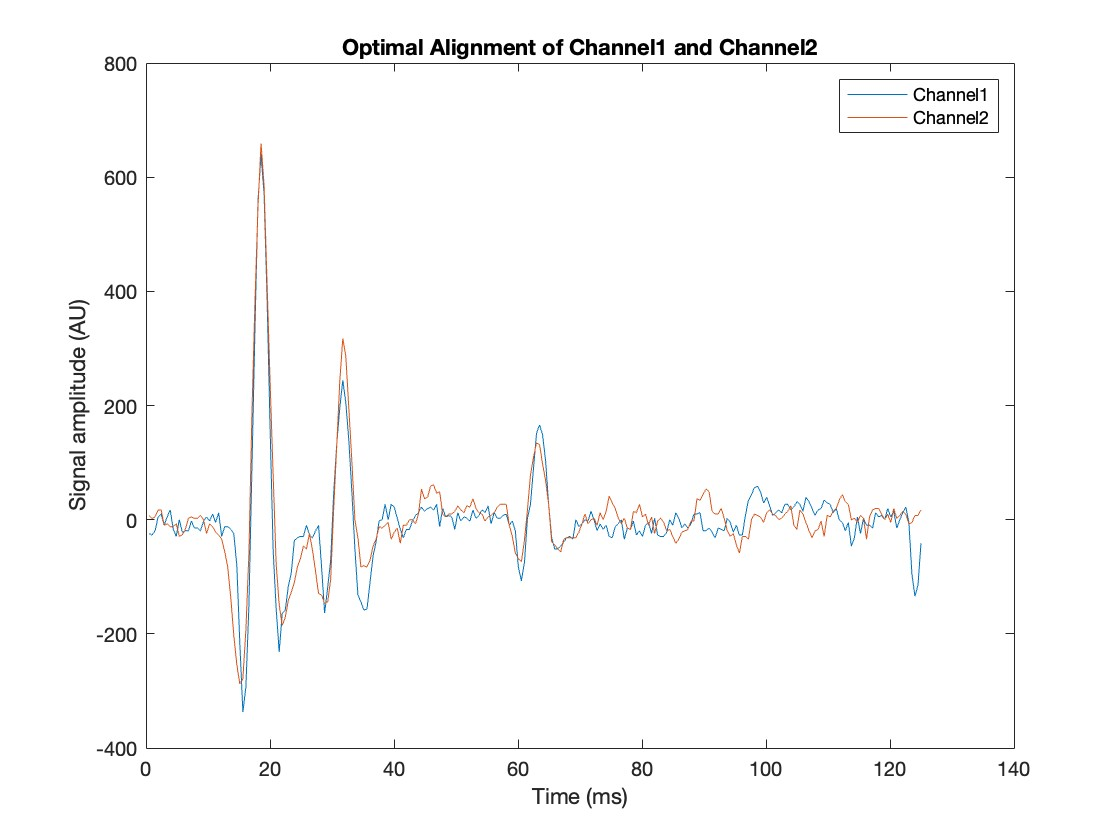
\includegraphics[width=\linewidth]{figure/figure_1.jpg}  
    \captionof{figure}{Optimal Alignment}
    \end{minipage}

    \vspace{0.5cm}

    \subsection{Estimation error with different downsampling factors(M)}
    
    \begin{minipage}{0.5\textwidth}  
    \centering  
    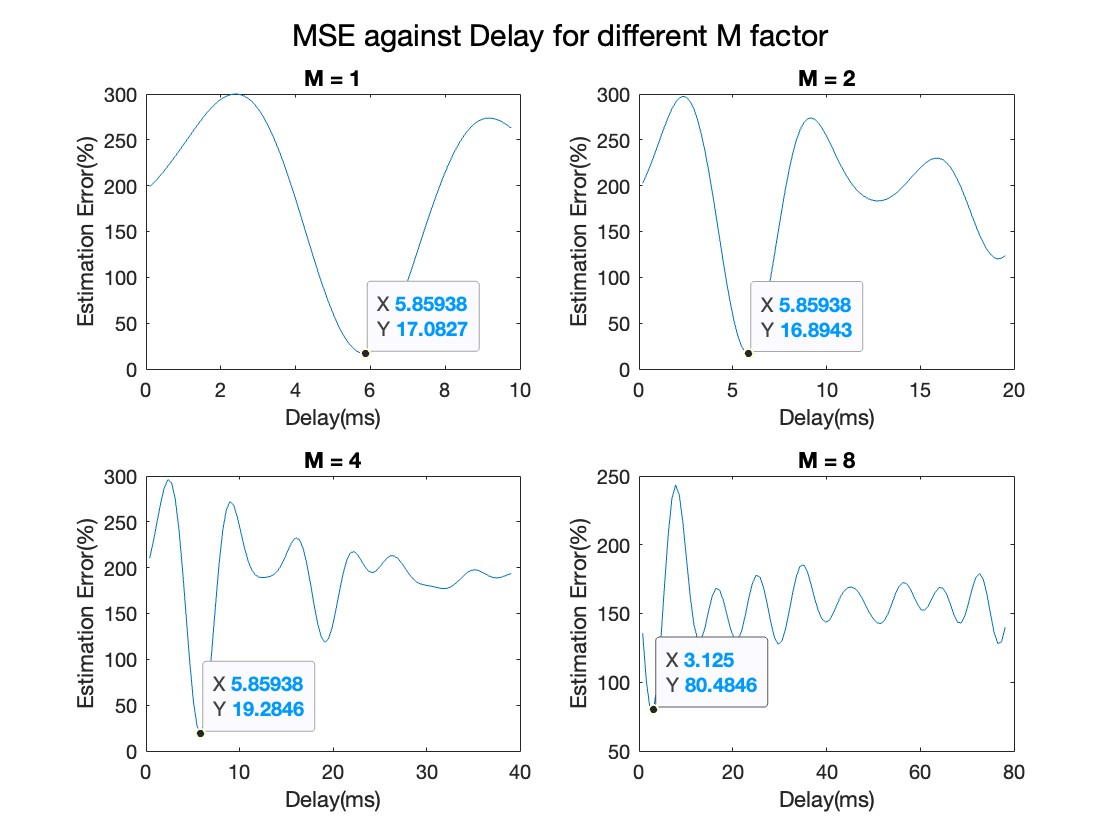
\includegraphics[width=\linewidth]{figure/figure_2.jpg}  
    \captionof{figure}{MSE against Delay for different M factor}
    \end{minipage}
    \hfill  
    \begin{minipage}{0.48\textwidth}   
    \begin{tabular}{|c|c|c|c|}  % Adjusted to 4 columns
    \hline
    M& Optimal Delay & Estimated Conduction Velocity & Optimal MSE \\
    \hline
    1 & \(5.86 \, \text{ms}\) & \(4.10 \, \text{m/s}\) & \(17.08\%\) \\
    2 & \(5.86 \, \text{ms}\) & \(4.10 \, \text{m/s}\) & \(16.89\%\) \\
    4 & \(5.86 \, \text{ms}\) & \(4.10 \, \text{m/s}\) & \(19.28\%\) \\
    8 & \(3.12 \, \text{ms}\) & \(7.68 \, \text{m/s}\) & \(80.48\%\) \\
    \hline
    \end{tabular}
    \captionof{table}{results with different downsampling factors}
    \vspace{0.3cm}
    Figure2 presents the estimated error, which is mean squared error (MSE), against delay for four different downsampling factors (1, 2, 4, 8). 
    For each downsampling factor M, the points of optimal delay are labeled (the x-axis represents the real-time domain). 
    \\
    Table2 report all detailed result for those four M.
    \\
    When M is set to 1, 2, or 4, both the optimal delay and the estimated conduction velocity remain constant at 5.86 ms and 4.10 m/s, respectively. 
    The optimal MSE is also quite similar, hovering around 17\%.
    \\
    When M increases to 8, minor fluctuations in both the optimal delay and conduction velocity are observed. 
    However, there is a significant jump in the optimal MSE, which escalates to 80.48\%. 
    This increase may be attributed to aliasing, indicating that the sampling frequency is below twice the signal bandwidth.
    \end{minipage}





    \newpage
    \section{Laboratory 2}
    \subsection{Average discharge rate}
    \begin{minipage}{0.4\textwidth}
    The figure beside illustrates the Discrete Fourier Transform applied to the discharge timing sequence of the first neuron. 
    The average discharge rate is highlighted in the figure, which corresponds to the second highest peak in the spectrum. 
    The second highest peak is chosen because the highest peak occurs at zero frequency, 
    which typically represents the mean value of the signal rather than its oscillatory frequency components.\\
    \\
    However, the frequency indicate in the figure is angular frequency, and it is a discrete frequency ($\omega$).
    Given sampling frequency is $2048Hz$, $T_s = \frac{1}{2048}s$. As $\omega = \Omega T_s$, the frequency can be find by:\\
    \[f = \frac{\Omega}{2 \pi} = \frac{\omega}{T_s} \times \frac{1}{2 \pi} = 0.0466175 \times 2048 \times \frac{1}{2 \pi} \approx 15.19 Hz\]
    \end{minipage}
    \hfill
    {\begin{minipage}{0.5\textwidth}
    \centering
    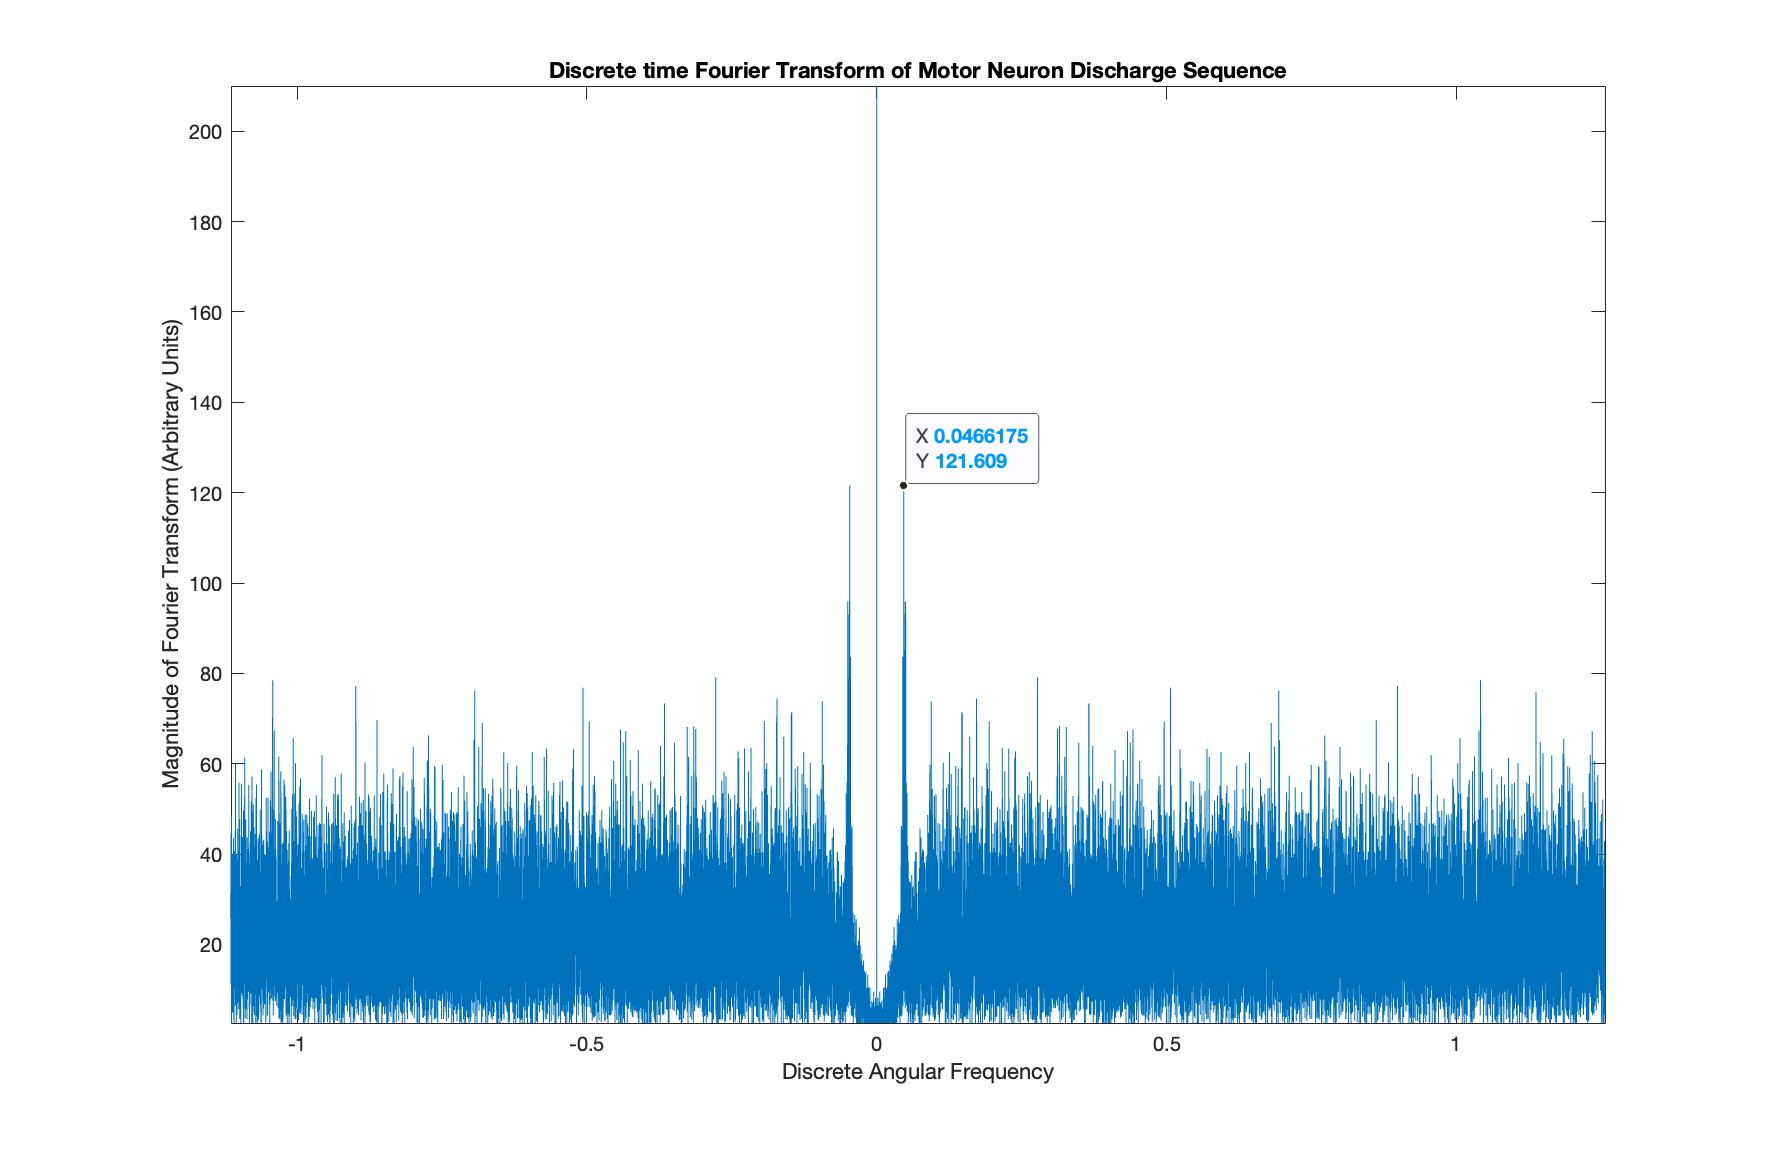
\includegraphics[width=\linewidth]{figure/figure_3.jpg}
    \captionof{figure}{Discrete Fourier Transform of Motor Neuron Discharge Sequence}
    \end{minipage}}

    \subsection{Torque and EMG envelopes with different filter length}
    \begin{minipage}{0.6\textwidth}
    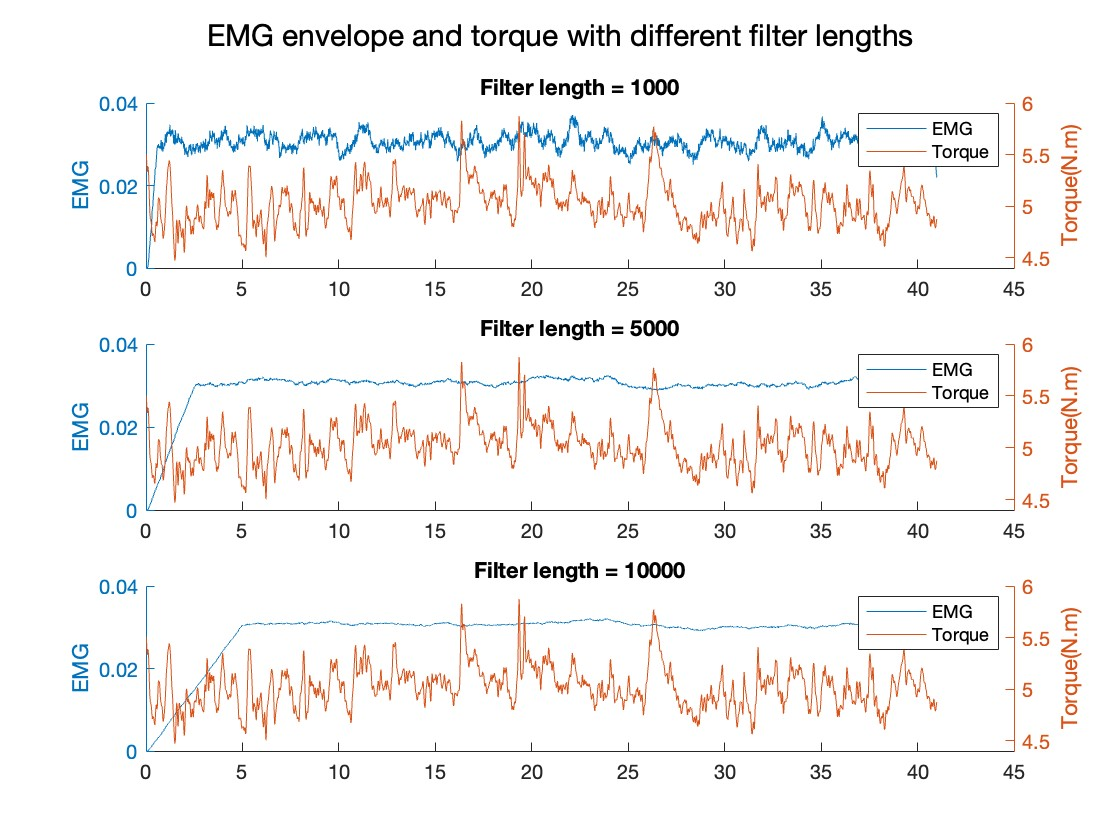
\includegraphics[width=\linewidth]{figure/figure_4.jpg}
    \captionof{figure}{EMG envelopes and torque with different filter lengths}
    \end{minipage}
    \begin{minipage}{0.5\textwidth}
        Average moving filter:
        \[ H(e^{j\omega}) = \frac{1}{M_2 +1} \frac{\sin[\omega \frac{M_2 + 1}{2}]}{\sin(\frac{\omega}{2})} e^{j\omega\frac{M_2}{2}}\] 
        By applying an average moving filter with three different lengths ($M_2 = 1000, 5000, 10000$) to the generated EMG signal, we can generate a plot (Figure 4).

The frequency responses in Figures 5, 6, and 7 represent the frequency responses of the three different values of $M_2$. These responses reveal that an increase in $M_2$ results in the filter having a lower cut-off frequency, which explains why the EMG signal appears smoother.
    \end{minipage}

    {
    \centering
    \begin{minipage}{0.3\textwidth}
    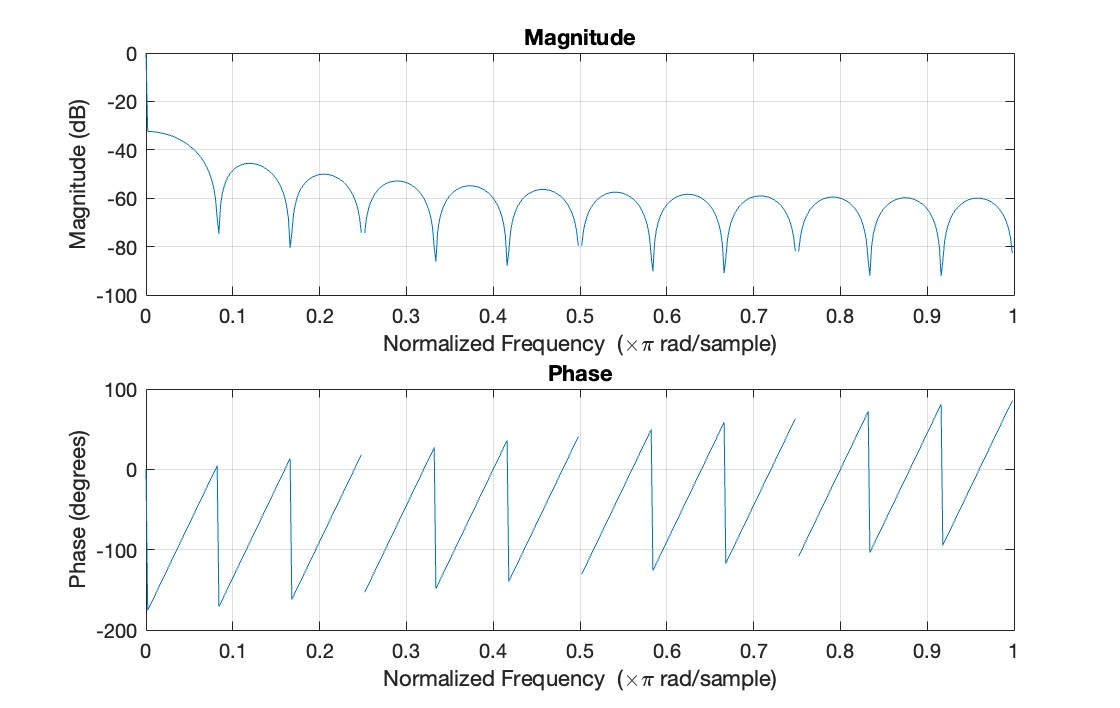
\includegraphics[width=\linewidth]{figure/filter_length_1000.jpg}
    \captionof{figure}{filter length = 1000}
    \end{minipage}
    \begin{minipage}{0.3\textwidth}
    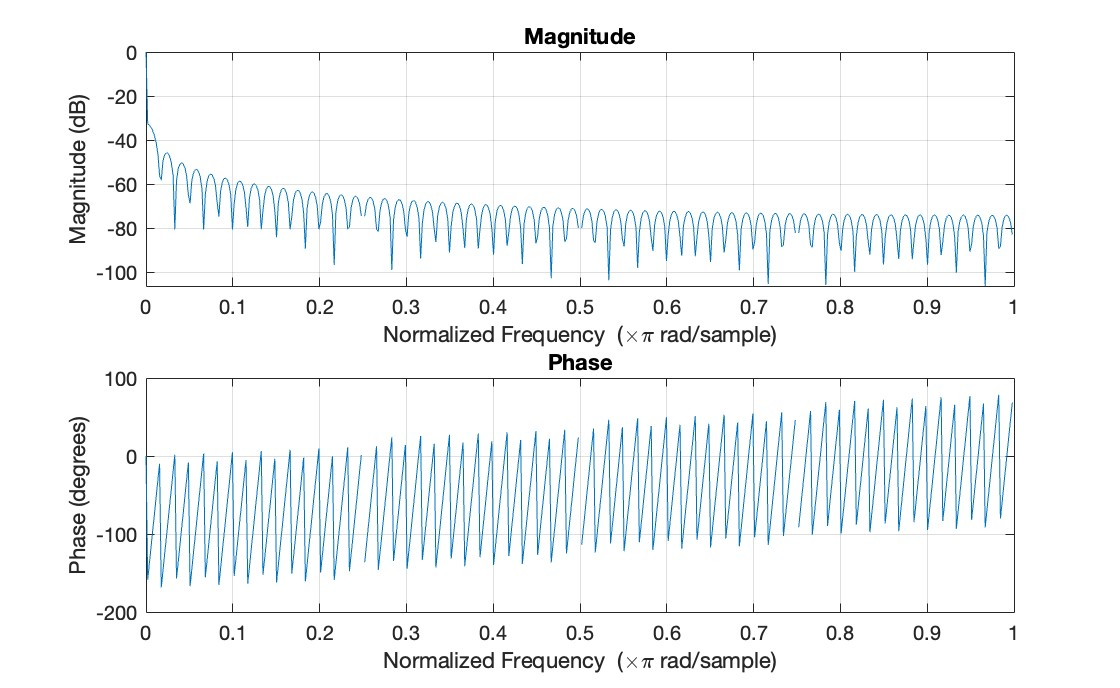
\includegraphics[width=\linewidth]{figure/filter_length_5000.jpg}
    \captionof{figure}{filter length = 5000}
    \end{minipage}
    \begin{minipage}{0.3\textwidth}
    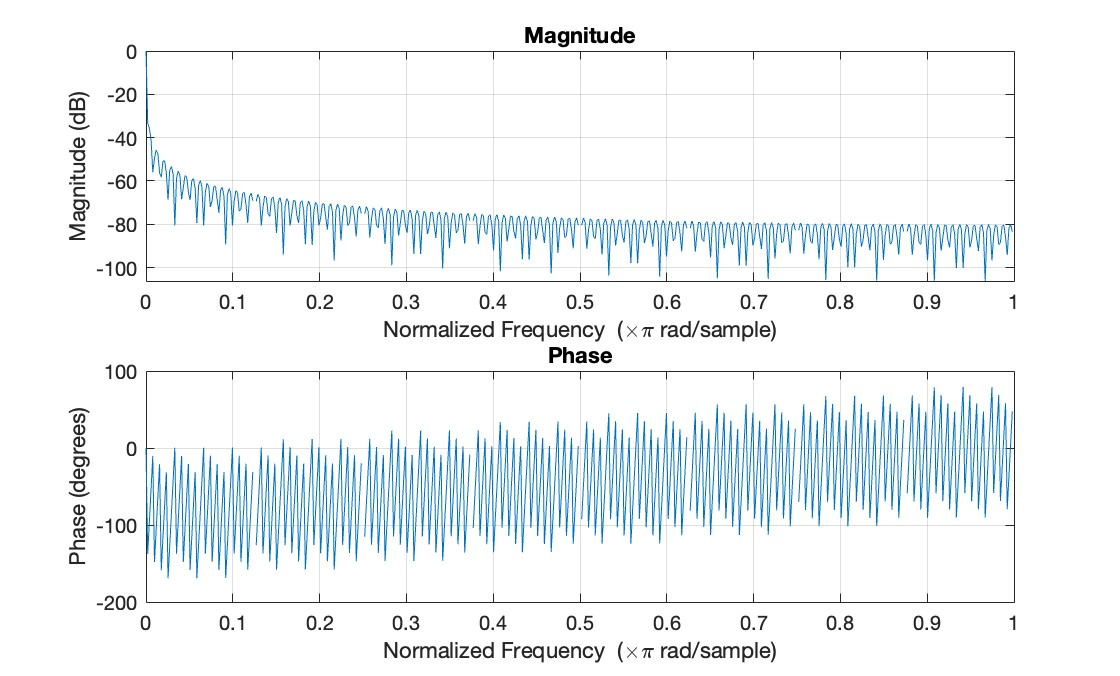
\includegraphics[width=\linewidth]{figure/filter_length_10000.jpg}
    \captionof{figure}{filter length = 10000}
    \end{minipage}}
    



    \newpage
    \section{Laboratory 3}
    \subsection{Power Spectral Density(PSD) of different signal duration}
    Figure 8 illustrates the PSD of the EEG signal for three different durations (1s, 5s, 15s). 
    The peak amplitude increased as the signal duration changed from 1s to 5s, 
    but it did not exhibit a significant increase from 5s to 15s.

    \[PSD[k] = \frac{1}{N}|\sum_{n=0}^{N-1}x[n]e^{-j2\pi k n/N}|^2\]
    Based on the formula provided earlier, a more dominant frequency will exhibit a peak in the PSD graph. 
    The presence of additional peaks with increasing signal duration may be attributed to the likelihood that longer signals encompass a greater variety of frequencies.
    
    {\centering
    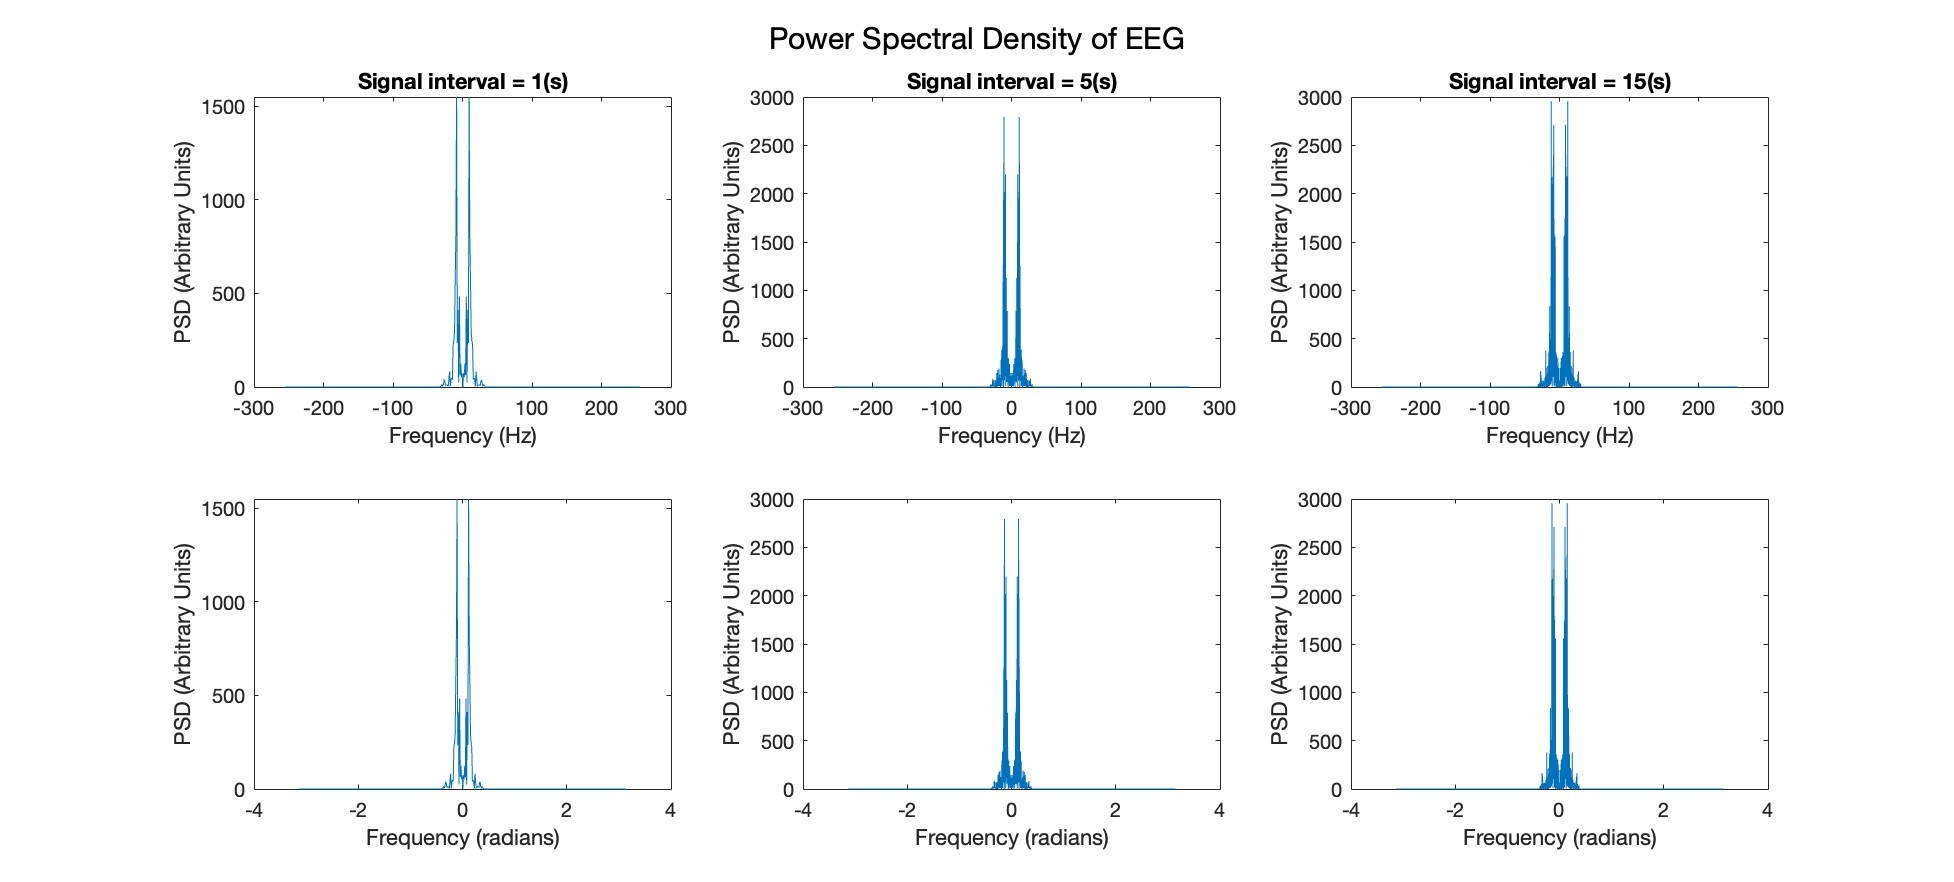
\includegraphics[width=\linewidth]{figure/figure_8.jpg}
    \captionof{figure}{PSDs with different signal duration}}

    \subsection{Power percentage of different frequency bands in EEG signal}

    The EEG signal have 5 different bands, having different frequency range. 
    There are Delta (0.5 $\leq$ f $\leq$ 4 Hz), Theta (4 $\leq$ f $\leq$ 8 Hz), Alpha (8 $\leq$ f $\leq$ 13 Hz), Beta (13 $\leq$ f $\leq$ 30 Hz), and Gamma (30 $\leq$f $\leq$ 42 Hz). 
    The power percentage is calculated from PSD and results is shown in Table3.
    \\

    {\centering
    \begin{tabular}{|c|c|c|c|c|c|}  % Adjusted to 4 columns
    \hline
    Duration(s)&Delta(\%)&Theta(\%)&Alpha(\%)&Beta(\%)&Gamma(\%)\\
    \hline
    1 &4.5036&17.6267&62.0336&15.3889&0.4117\\
    5 &4.5897&16.4315&64.2288&14.3339&0.2527\\
    15 &3.4897&16.3561&62.4016&17.3467&0.2050\\
    \hline
    \end{tabular}
    \captionof{table}{Different bands' power percentage}}
    \vspace{0.1cm}
    
    The power percentage didn't change significantly with different signal durations. Noticeably,
     the Alpha band is the most dominant frequency band,
     Beta and Theta are the second most active bands.

    \end{document}